\question*{
    Hardware
}

\begin{arabicparts}
    \questionpart
    \textbf{16 MHz.} The frequency of the clock was found to
    be 16 MHz from the datasheet. 

    \questionpart
    \textbf{16/20 MHz.} Data differs between different datasheets
    I checked. 

    \questionpart
    \textbf{Power.} Higher voltages are required to run at higher frequncies c.f. Fig \ref{subfig:voltfreq},
    presumably due to loads causing reduction in voltage and it becoming 
    harder to distinguish between low and high. At the same time, the current
    required increases as well (Fig. \ref{subfig:currfreq}). Thus, the net increase 
    in power will limit the frequency at which we can drive the chip due to thermal
    as well as electric constraints. Thermal should set in first. If you were able
    to provide external cooling say witha  fan, electrical limitations would take over 
    soon.

    \questionpart
    Setup done.

    \begin{figure}[ht]
        \centering
        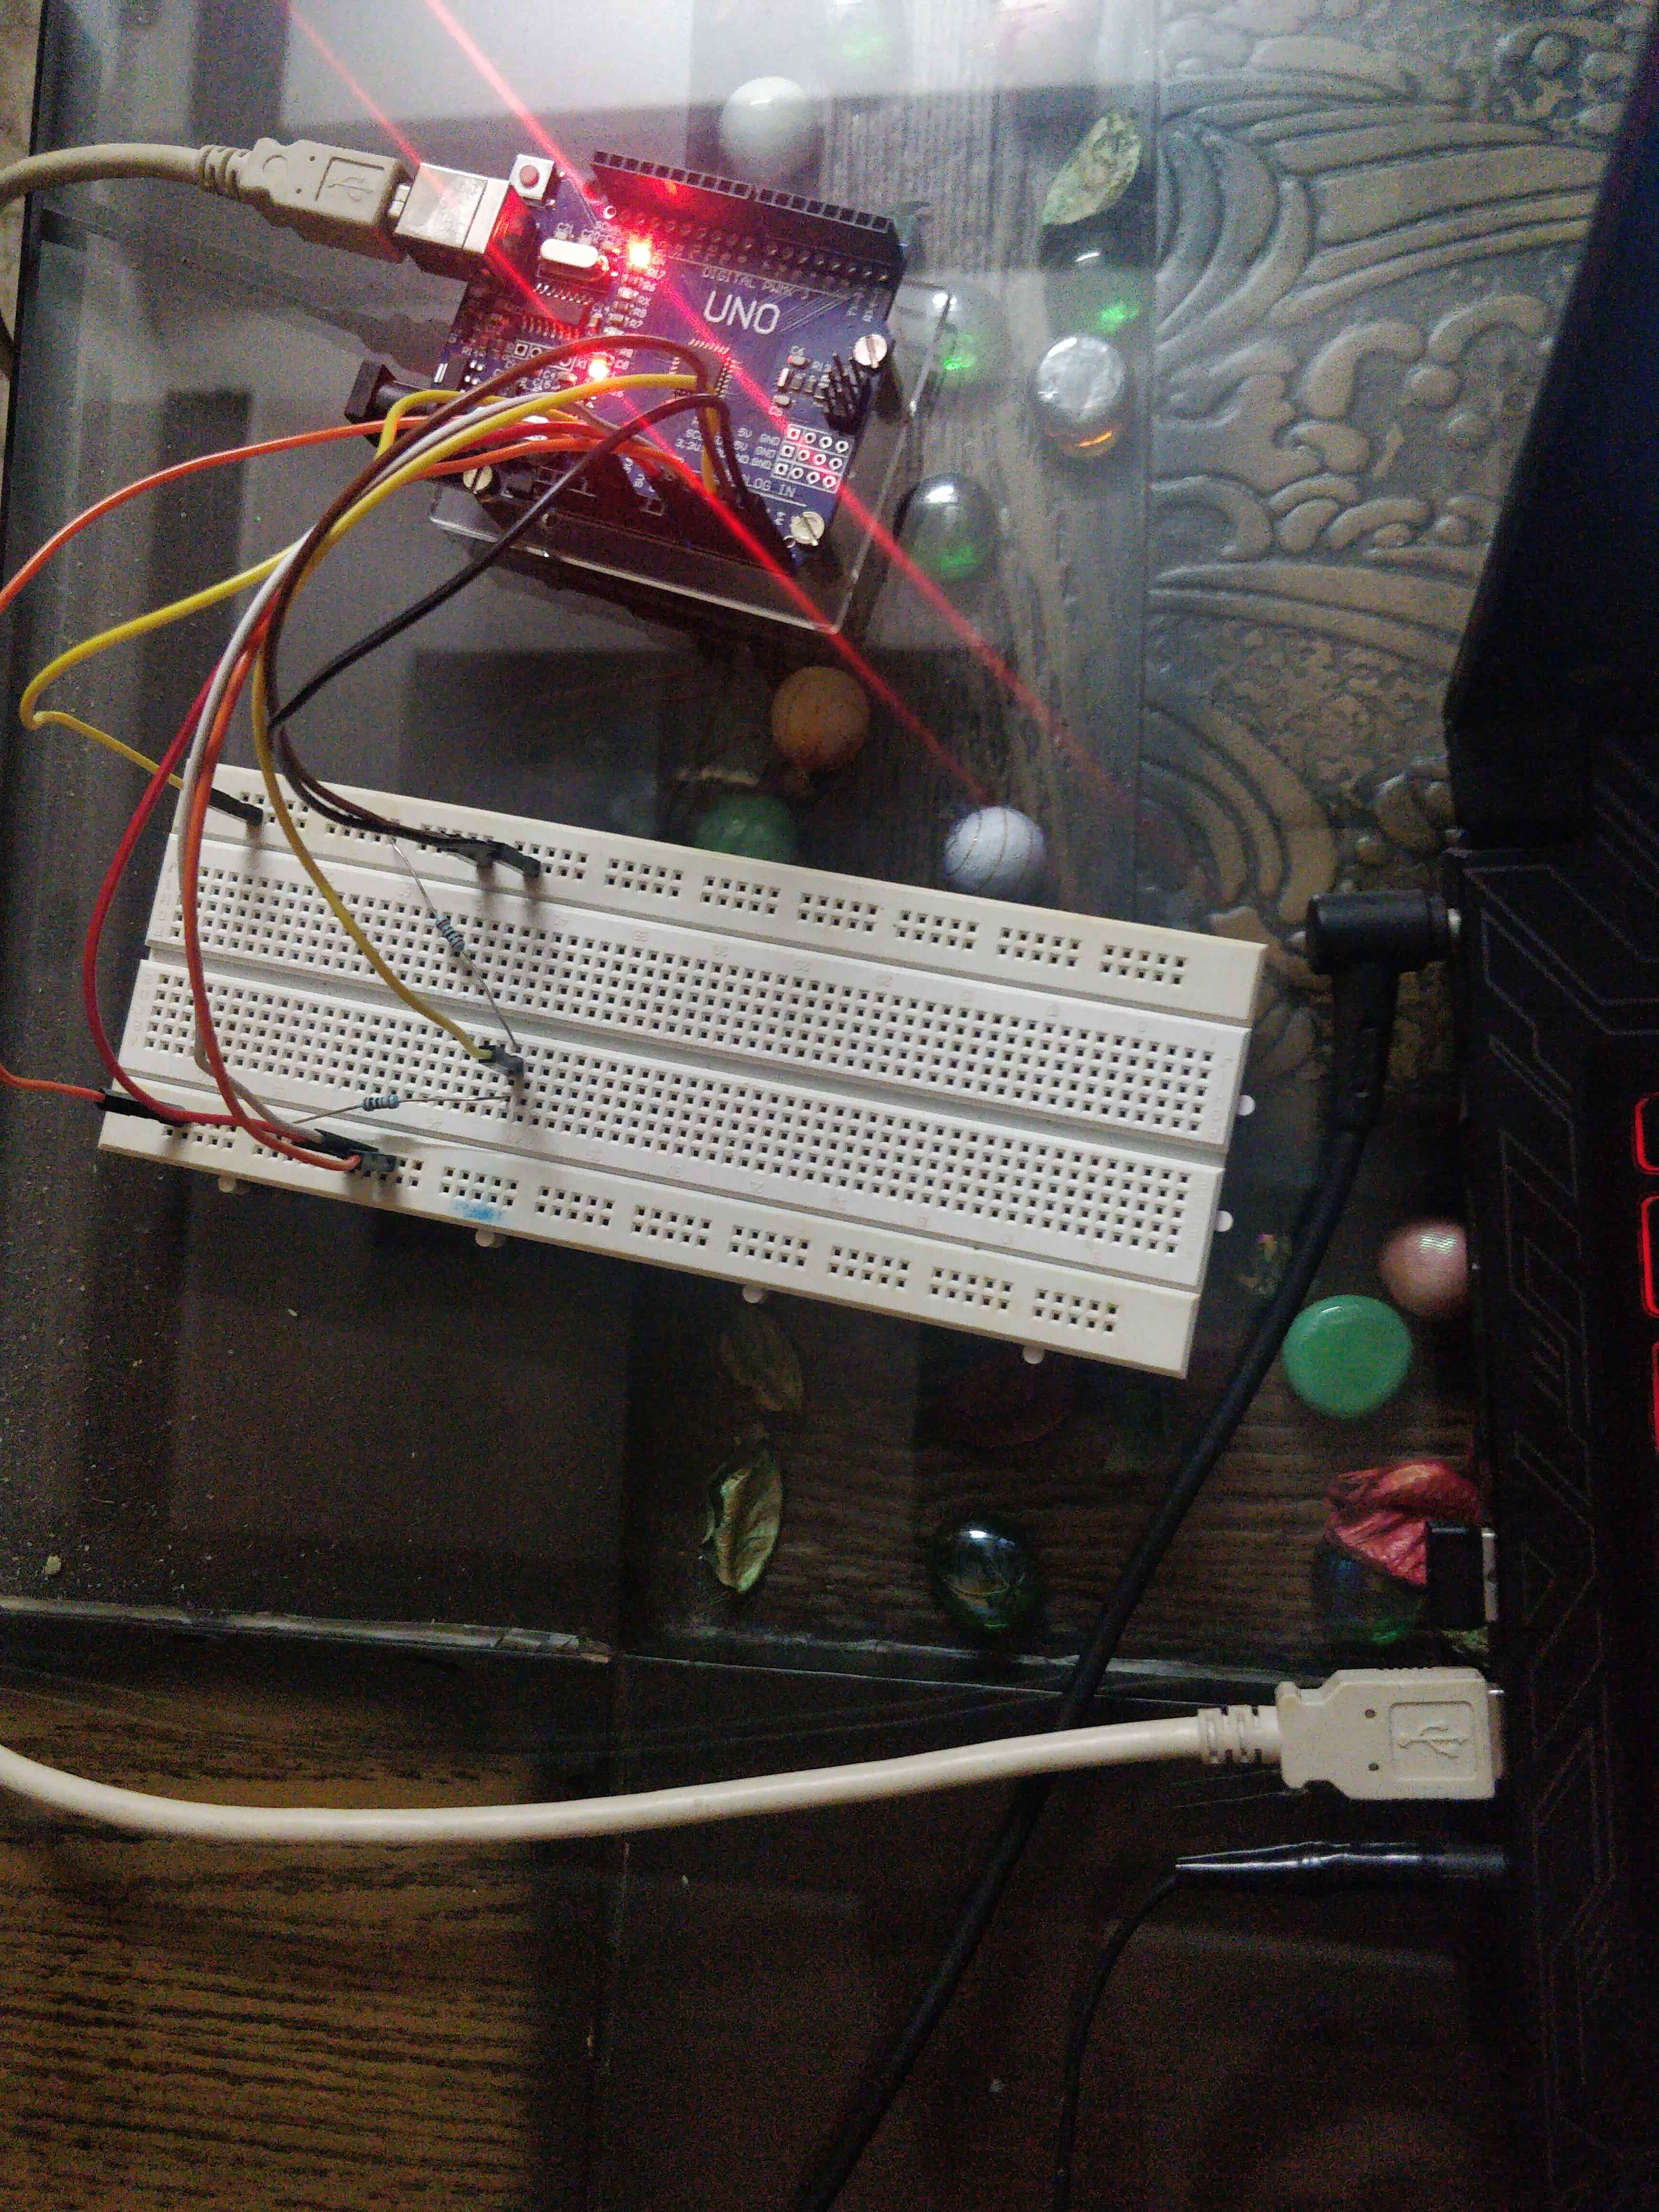
\includegraphics[width=0.5\textwidth]{fig/arduinoconnected-min.jpg}
        \caption{Arduino connected to laptop}
        \label{fig:arduinoconnected}
    \end{figure}


    \begin{figure}[!hp]
        \centering
        \begin{subfigure}[b]{0.83\textwidth}
            \centering
            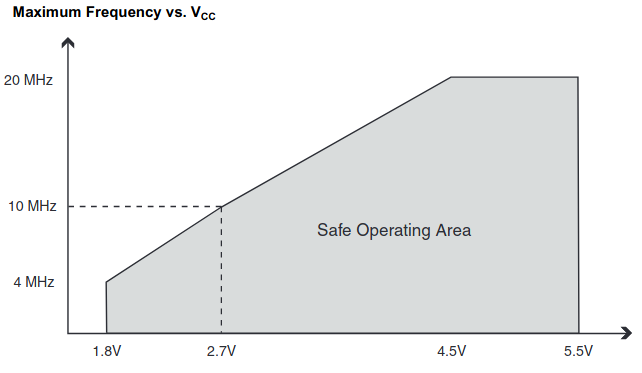
\includegraphics[width=\textwidth]{fig/voltfreq.png}
            \caption{$V-f$}
            \label{subfig:voltfreq}
        \end{subfigure}
        %
        \begin{subfigure}[b]{0.9\textwidth}
            \centering
            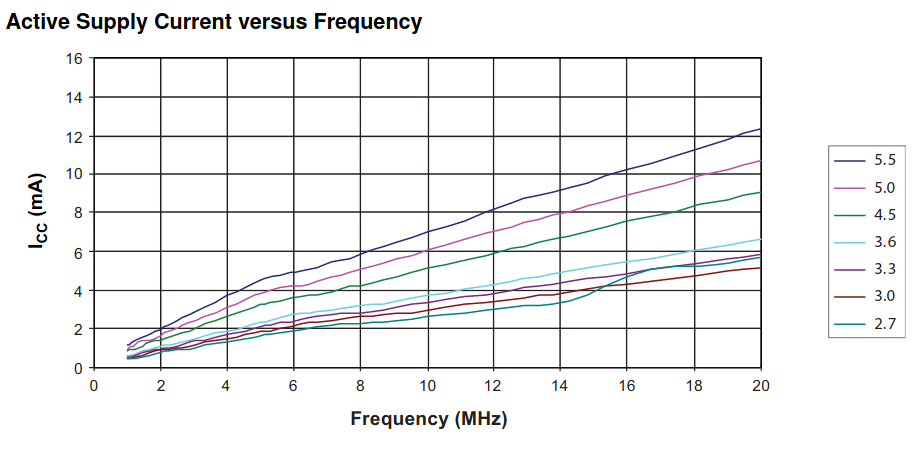
\includegraphics[width=\textwidth]{fig/currfreq.png}
            \caption{$f-I$}
            \label{subfig:currfreq}
        \end{subfigure}        
        %
        \captionsetup{justification=centering}
        \caption{Graphs for electric constraints with frequency \\
        Taken from \url{https://www.microchip.com/wwwproducts/en/ATmega328p}}
        \label{fig:elecfreq}
    \end{figure}


\end{arabicparts}